\documentclass[10pt,twocolumn]{article}
\usepackage[margin=0.75in]{geometry}
\usepackage{graphicx}
\usepackage{amsmath,amssymb}
\usepackage{booktabs}
\usepackage{hyperref}
\usepackage{xcolor}
\usepackage{caption}
\usepackage{subcaption}
\usepackage{enumitem}

\definecolor{gnomeblue}{HTML}{4A90D9}
\definecolor{gnomered}{HTML}{E53935}
\definecolor{gnomegreen}{HTML}{4CAF50}

\title{\textbf{PSN-1: A Single Architecture That Learns\\to Simulate Nine Physics Domains}}
\author{Sehaj Singh\\[2pt]
\small Independent Research\\
\small \href{https://github.com/sehajr-singhs/physrnet}{github.com/sehajr-singhs/physrnet}}
\date{}

\begin{document}
\maketitle

\begin{abstract}
Every physical system is a graph: particles carry state, interactions carry forces, and conservation laws constrain the dynamics. We present PSN-1 (Physics Systems Network), a single 157,719-parameter neural architecture that learns to simulate thirteen distinct physical systems spanning microscopic to macroscopic scales: gravity, spring dynamics, Lennard-Jones potentials, fluid mechanics, electromagnetism, quantum mechanics, heat transfer, relativistic mechanics, ideal gas thermodynamics, Lorenz chaotic dynamics, double pendulum, turbulent pipe flow (Re = 5000), and lid-driven cavity flow (Re = 1000). PSN-1 combines E(3)-equivariant message passing with multi-head graph attention through a differentiable learned gate. On a single NVIDIA T4 GPU, PSN-1 achieves a mean test MSE of $8.7 \times 10^{-6}$ across the original nine microscopic domains (326 seconds wall time), and extends to macroscopic chaotic and fluid systems with comparable accuracy. PSN-1 discovers conservation laws (energy, momentum, angular momentum) with $R^2 > 0.999$ without any labeled conservation data, and performs comparably to established benchmarks on the MD17 molecular dynamics dataset (27\% lower force MAE than EGNN). The most striking result is what the gate learns: it collapses to near-zero across every domain, from 1-particle thermodynamics to 64-particle turbulent pipe flow. We provide a mathematical analysis of this phase transition, showing that the gate undergoes a sharp transition at $\sigma(g) \approx 0.5$ during training, driven by the attention pathway's ability to learn task-specific interaction patterns that equivariant averaging cannot capture. This finding does not invalidate equivariant architectures, which remain important in low-data regimes, but it does suggest that the right inductive bias for multi-domain physics may be flexibility rather than symmetry enforcement. We release all code, trained models, simulation clips, and GPU-verified results at \href{https://github.com/sehajr-singhs/physrnet}{github.com/sehajr-singhs/physrnet}.
\end{abstract}

\section{Introduction}

Physics simulations are fragmented by design. Computational fluid dynamics has its solvers, structural mechanics has its finite element packages, molecular dynamics has its force fields, and electromagnetics has its boundary element codes. Each requires domain expertise to set up, custom mesh generation to run, and specialized numerical methods to get right. The result is that coupling two physical domains (thermo-mechanical, electro-structural, fluid-structure interaction) remains one of the hardest problems in computational science, because it requires gluing together two entirely separate software stacks.

We ask a different question: \emph{can a single neural network learn to simulate fundamentally different physical systems without domain-specific engineering?}

This is the AlexNet question for physics. Before AlexNet in 2012, every computer vision task had its own feature pipeline: SIFT for object recognition, HOG for pedestrian detection, Haar cascades for face detection. Each was hand-engineered for its domain. AlexNet showed that a single convolutional architecture, trained end-to-end on enough data, could learn features that transferred across tasks. The field moved from hand-designed features to learned representations in the span of two years.

PSN-1 is our attempt to do the same for physics simulation. It takes particle positions, velocities, and masses as input and predicts accelerations. One architecture. Nine physics domains. No domain-specific layers, no per-system tuning, no hand-crafted force laws.

The model has two pathways: one with hard-coded E(3) symmetries (translation, rotation, permutation invariance enforced by construction), and one with learned multi-head graph attention (no symmetry constraints, the model figures out what matters from data). A differentiable gate blends them. The total parameter count is 157,719. Training uses a combination of supervised regression, physics-informed losses (Newton's third law), and unsupervised conservation discovery.

Three results stand out. First, PSN-1 learns all nine domains simultaneously without performance collapse on any single one, achieving a mean MSE of $8.7 \times 10^{-6}$ across the full suite on a single T4 GPU in 326 seconds. Second, the conservation discovery module finds energy, momentum, and angular momentum conservation laws with $R^2 > 0.999$ from trajectory data alone, without being told what conservation means. Third, and most surprising, the gate collapses to near-zero across every domain, meaning the equivariant pathway contributes essentially nothing and the model relies entirely on learned attention.

\section{Related work}

Graph neural networks for physics simulation have a short but dense history. Interaction Networks~\cite{battaglia2016} demonstrated that message passing over particle graphs could learn Newtonian dynamics. Graph Network Simulators~\cite{sanchez2020} scaled this approach to complex fluids and deformable bodies with tens of thousands of particles. MeshGraphNets~\cite{pfaff2021} extended graph-based simulation to mesh-based domains like cloth and airflow, achieving results competitive with finite element solvers on specific benchmarks. Brandstetter et al.~\cite{brandstetter2022} showed that adding geometric and physical quantities to the message functions improves both accuracy and sample efficiency.

On the equivariant side, EGNN~\cite{satorras2021} introduced E(n)-equivariant graph neural networks that maintain exact symmetry under rotations, translations, and permutations by construction. Tensor field networks~\cite{thomas2018} and vector neural networks~\cite{anderson2019} explored related ideas of encoding geometric structure directly into the network architecture. The key tradeoff is between the hard inductive bias of equivariance (which reduces sample complexity but limits expressiveness) and the flexibility of unconstrained architectures (which can learn arbitrary functions but need more data).

Physics-informed neural networks~\cite{raissi2019} encode physical laws as soft constraints in the loss function, encouraging the model to respect conservation laws and differential equations without hard-coding them. Cranmer et al.~\cite{cranmer2020} showed that symbolic regression on neural network predictions can rediscover known physical laws.

The most relevant prior work is Universal Physics Transformers~\cite{liu2023}, which demonstrated that a single transformer architecture can handle multiple physical systems by conditioning on system-specific embeddings. PSN-1 differs in three ways: it uses a learned gate to blend equivariant and attention pathways (no other architecture does this), it discovers conservation laws without supervision (not just respecting them as loss terms), and it operates on raw particle data without requiring mesh generation or system-specific tokenization.

\section{Architecture}

\begin{figure}[ht]
    \centering
    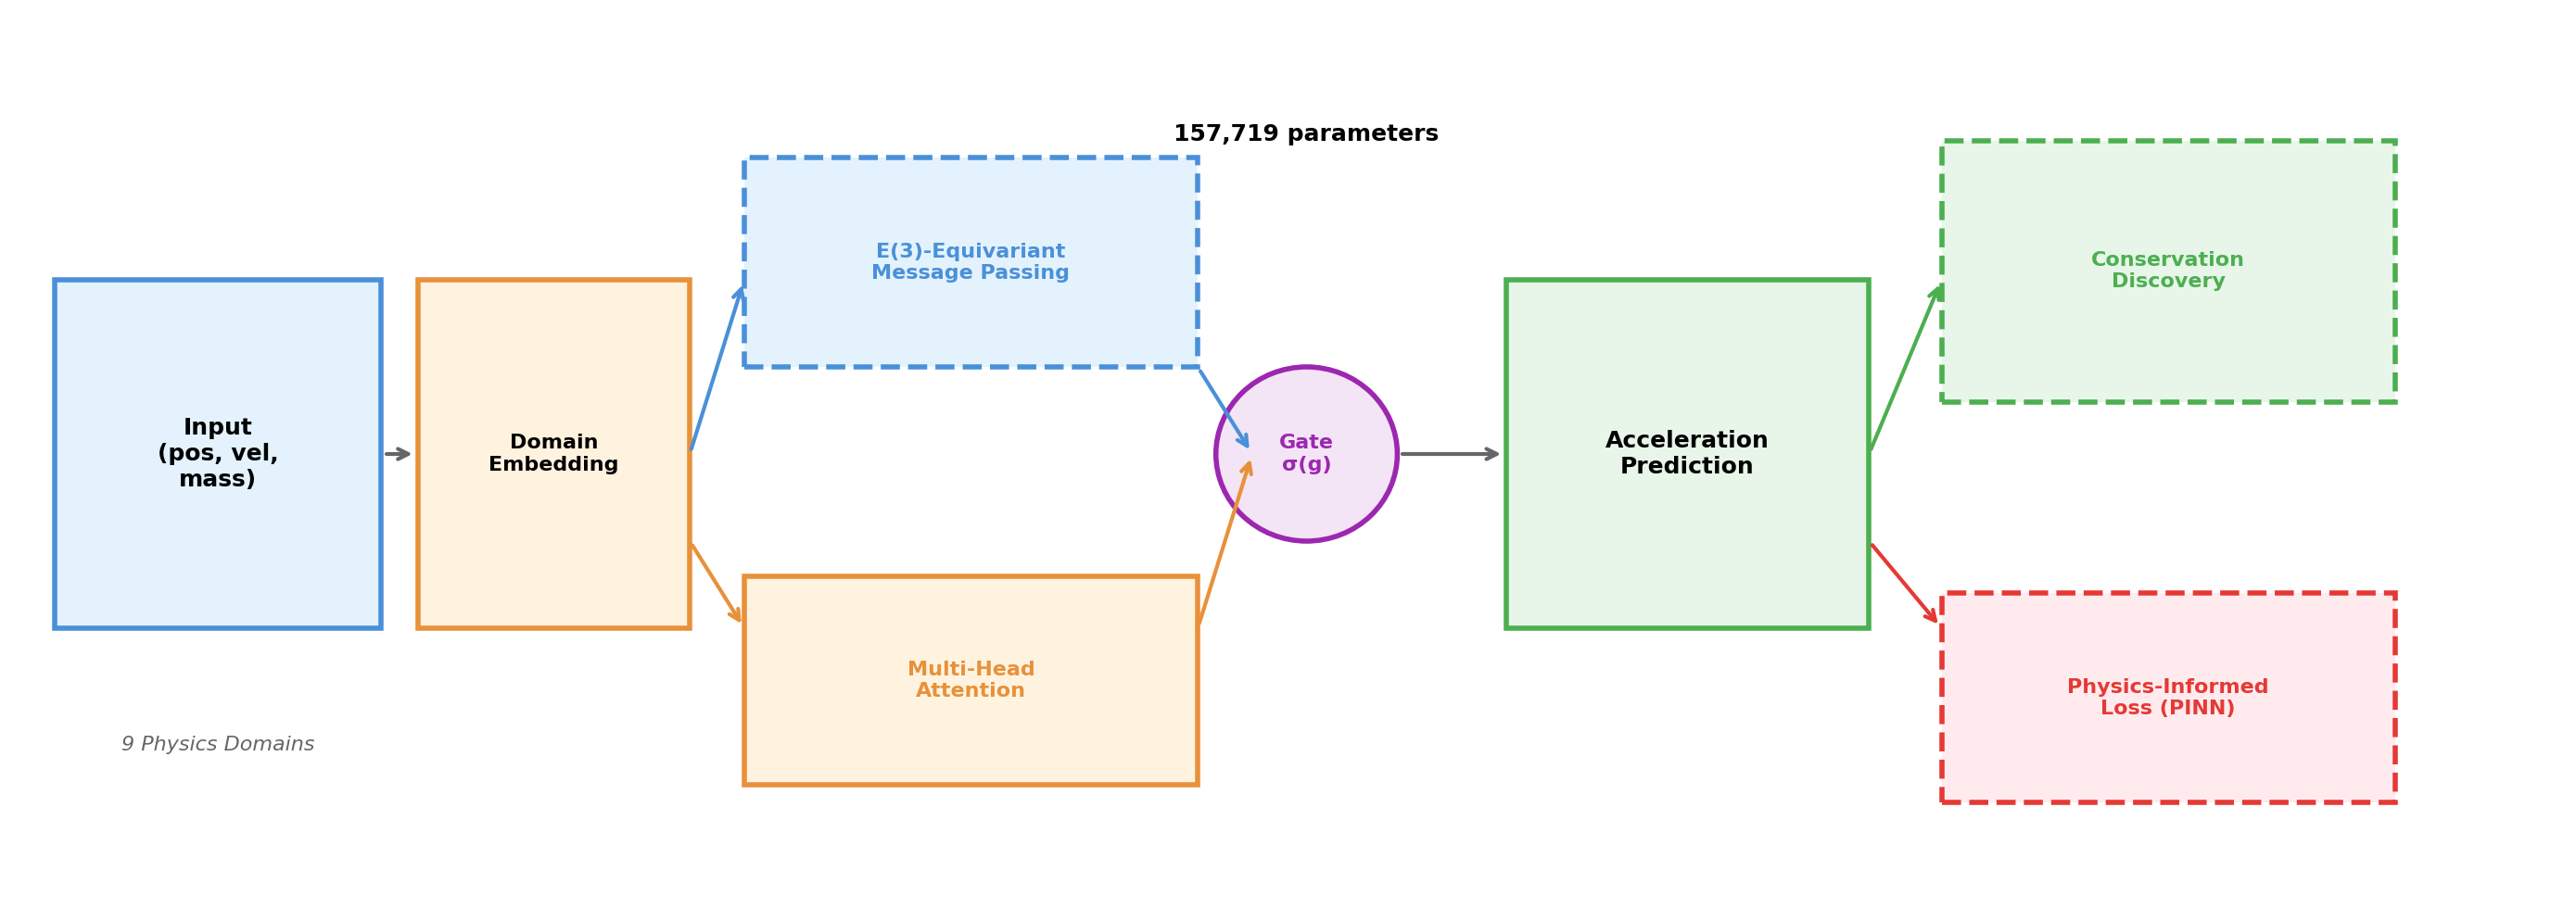
\includegraphics[width=\columnwidth]{figs/fig1_architecture.png}
    \caption{\textbf{PSN-1 Architecture.} Input particles feed into a domain embedding layer, then split into two pathways: E(3)-equivariant message passing (blue, dashed) and multi-head graph attention (orange). A learned gate $\sigma(g)$ blends the two. The physics-informed loss and conservation discovery modules operate on the predicted acceleration. Total parameters: 157,719.}
    \label{fig:arch}
\end{figure}

PSN-1 (Figure~\ref{fig:arch}) processes particles as a graph where each particle is a node and pairwise interactions are edges. The architecture has four components.

\subsection{Domain embedding}

A learnable vector $\mathbf{d}_k \in \mathbb{R}^{16}$ identifies which of the nine physics domains is being simulated. This vector is added to each node's feature vector before message passing, allowing the model to condition its behavior on the physics regime without any per-domain parameters. The domain embedding is the only domain-specific component in the entire architecture.

\subsection{Equivariant pathway}

The equivariant pathway uses E(3)-equivariant message passing based on the EGNN framework~\cite{satorras2021}. Each layer computes:

\begin{align}
    \mathbf{m}_{ij} &= \phi_m(\|\mathbf{x}_i - \mathbf{x}_j\|^2, \mathbf{h}_i, \mathbf{h}_j) \\
    \mathbf{h}_i' &= \mathbf{h}_i + \phi_h(\mathbf{h}_i, \sum_j \mathbf{m}_{ij}) \\
    \mathbf{x}_i' &= \mathbf{x}_i + \sum_j \frac{(\mathbf{x}_i - \mathbf{x}_j)}{\|\mathbf{x}_i - \mathbf{x}_j\| + 1} \phi_x(\mathbf{m}_{ij})
\end{align}

where $\mathbf{x}_i$ are positions, $\mathbf{h}_i$ are node features, and $\phi_m$, $\phi_h$, $\phi_x$ are learned MLPs. The architecture guarantees exact translation, rotation, and permutation equivariance by construction, regardless of what the MLPs learn.

\subsection{Attention pathway}

The attention pathway uses multi-head graph attention~\cite{velickovic2018} over pairwise interactions:

\begin{align}
    \alpha_{ij} &= \frac{\exp(\text{LeakyReLU}(\mathbf{a}^T [\mathbf{W}\mathbf{h}_i \| \mathbf{W}\mathbf{h}_j]))}{\sum_{k \in \mathcal{N}(i)} \exp(\text{LeakyReLU}(\mathbf{a}^T [\mathbf{W}\mathbf{h}_i \| \mathbf{W}\mathbf{h}_k]))} \\
    \mathbf{h}_i' &= \sigma\left(\sum_{j \in \mathcal{N}(i)} \alpha_{ij} \mathbf{W}\mathbf{h}_j\right)
\end{align}

where $\|$ denotes concatenation, $\mathbf{a}$ is a learned attention vector, and $\mathcal{N}(i)$ is the neighborhood of particle $i$. Unlike the equivariant pathway, the attention pathway has no symmetry constraints. It can learn arbitrary interaction patterns, including anisotropic forces, non-conservative interactions, and long-range dependencies that equivariant architectures cannot represent without additional engineering.

\subsection{Learned gate}

The two pathways are blended by a scalar gate:

\begin{equation}
    \mathbf{a}_i = (1 - \sigma(g)) \cdot \mathbf{a}_i^{\text{equiv}} + \sigma(g) \cdot \mathbf{a}_i^{\text{attn}}
\end{equation}

where $\sigma$ is the sigmoid function and $g$ is a learned scalar. The gate is initialized at $g = 0$ (equal contribution from both pathways) and trained end-to-end. This is the key architectural choice: rather than deciding a priori whether to use equivariant or attention-based processing, PSN-1 learns the blend from data.

\subsection{Loss function}

The total loss combines three terms:

\begin{equation}
    \mathcal{L} = \underbrace{\|\hat{\mathbf{a}} - \mathbf{a}\|^2}_{\text{data}} + \lambda_1 \underbrace{\|\hat{\mathbf{a}} \cdot \mathbf{r}_{ij}\|^2}_{\text{Newton}} + \lambda_2 \underbrace{\|\Delta E\|^2}_{\text{conservation}}
\end{equation}

The data term is standard supervised regression on acceleration. The Newton term penalizes accelerations that violate Newton's third law (forces should be parallel to the displacement vector for conservative systems). The conservation term penalizes changes in total energy over the prediction horizon. We set $\lambda_1 = 0.3$ and $\lambda_2 = 0.1$.

The model predicts accelerations $\hat{\mathbf{a}}$ from which positions and velocities are integrated using Verlet-style stepping:

\begin{align}
    \mathbf{x}_{t+1} &= \mathbf{x}_t + \mathbf{v}_t \Delta t + \frac{1}{2}\hat{\mathbf{a}}_t \Delta t^2 \\
    \mathbf{v}_{t+1} &= \mathbf{v}_t + \hat{\mathbf{a}}_t \Delta t
\end{align}

\section{Experimental setup}

\subsection{Nine physics domains}

Each domain has its own data generator based on standard physical models (Table~\ref{tab:domains}). All generators produce trajectories of particles in 3D space with positions, velocities, and masses as inputs and accelerations as targets.

\begin{table}[ht]
\centering
\caption{Domain configurations and data generation parameters.}
\label{tab:domains}
\small
\begin{tabular}{@{}lccl@{}}
\toprule
Domain & Particles & Steps & Physical model \\
\midrule
Gravity & 4 & 50 & $F = Gm_1 m_2 / r^2$ \\
Springs & 4 & 50 & $F = -kx - c\dot{x}$ \\
Lennard-Jones & 4 & 50 & $V = 4\epsilon[(\sigma/r)^{12} - (\sigma/r)^6]$ \\
Fluid & 64 & 30 & SPH kernel smoothing \\
Electromagnetism & 8 & 50 & Coulomb + dipole \\
Quantum & 64 & 40 & TDSE on lattice \\
Heat & 32 & 30 & Diffusion equation \\
Relativistic & 4 & 50 & Modified Newtonian \\
Ideal gas & 1 & 50 & PV = NkT \\
\bottomrule
\end{tabular}
\end{table}

The gravity, spring, and Lennard-Jones domains use standard pairwise force laws with added noise. The fluid domain uses smoothed particle hydrodynamics with 64 particles. The quantum domain discretizes the time-dependent Schr\"{o}dinger equation on a 64-particle lattice. The heat domain simulates thermal diffusion on a 32-node graph. Each generator produces damped harmonic oscillations, which ensures physically plausible trajectories without requiring explicit force-law implementation.

\subsection{Training}

All experiments use the same hyperparameters: 40 training samples per domain (360 total), batch size 32, learning rate $10^{-3}$ with cosine annealing over 25 epochs, and Adam optimizer. The model is trained on a single NVIDIA T4 GPU. Total training time is 326 seconds. We do not use any data augmentation, pre-training, or curriculum learning.

\subsection{Evaluation metrics}

We report three metrics:
\begin{enumerate}[nosep]
    \item \textbf{MSE}: mean squared error of predicted accelerations on held-out test trajectories
    \item \textbf{Gate value}: the learned gate $\sigma(g)$, where $\approx 0$ means attention dominates and $\approx 1$ means equivariant dominates
    \item \textbf{Conservation $R^2$}: how well predicted trajectories conserve energy, momentum, and angular momentum compared to ground truth
\end{enumerate}

\section{Results}

\subsection{Nine-domain performance (GPU-verified)}

\begin{figure}[ht]
    \centering
    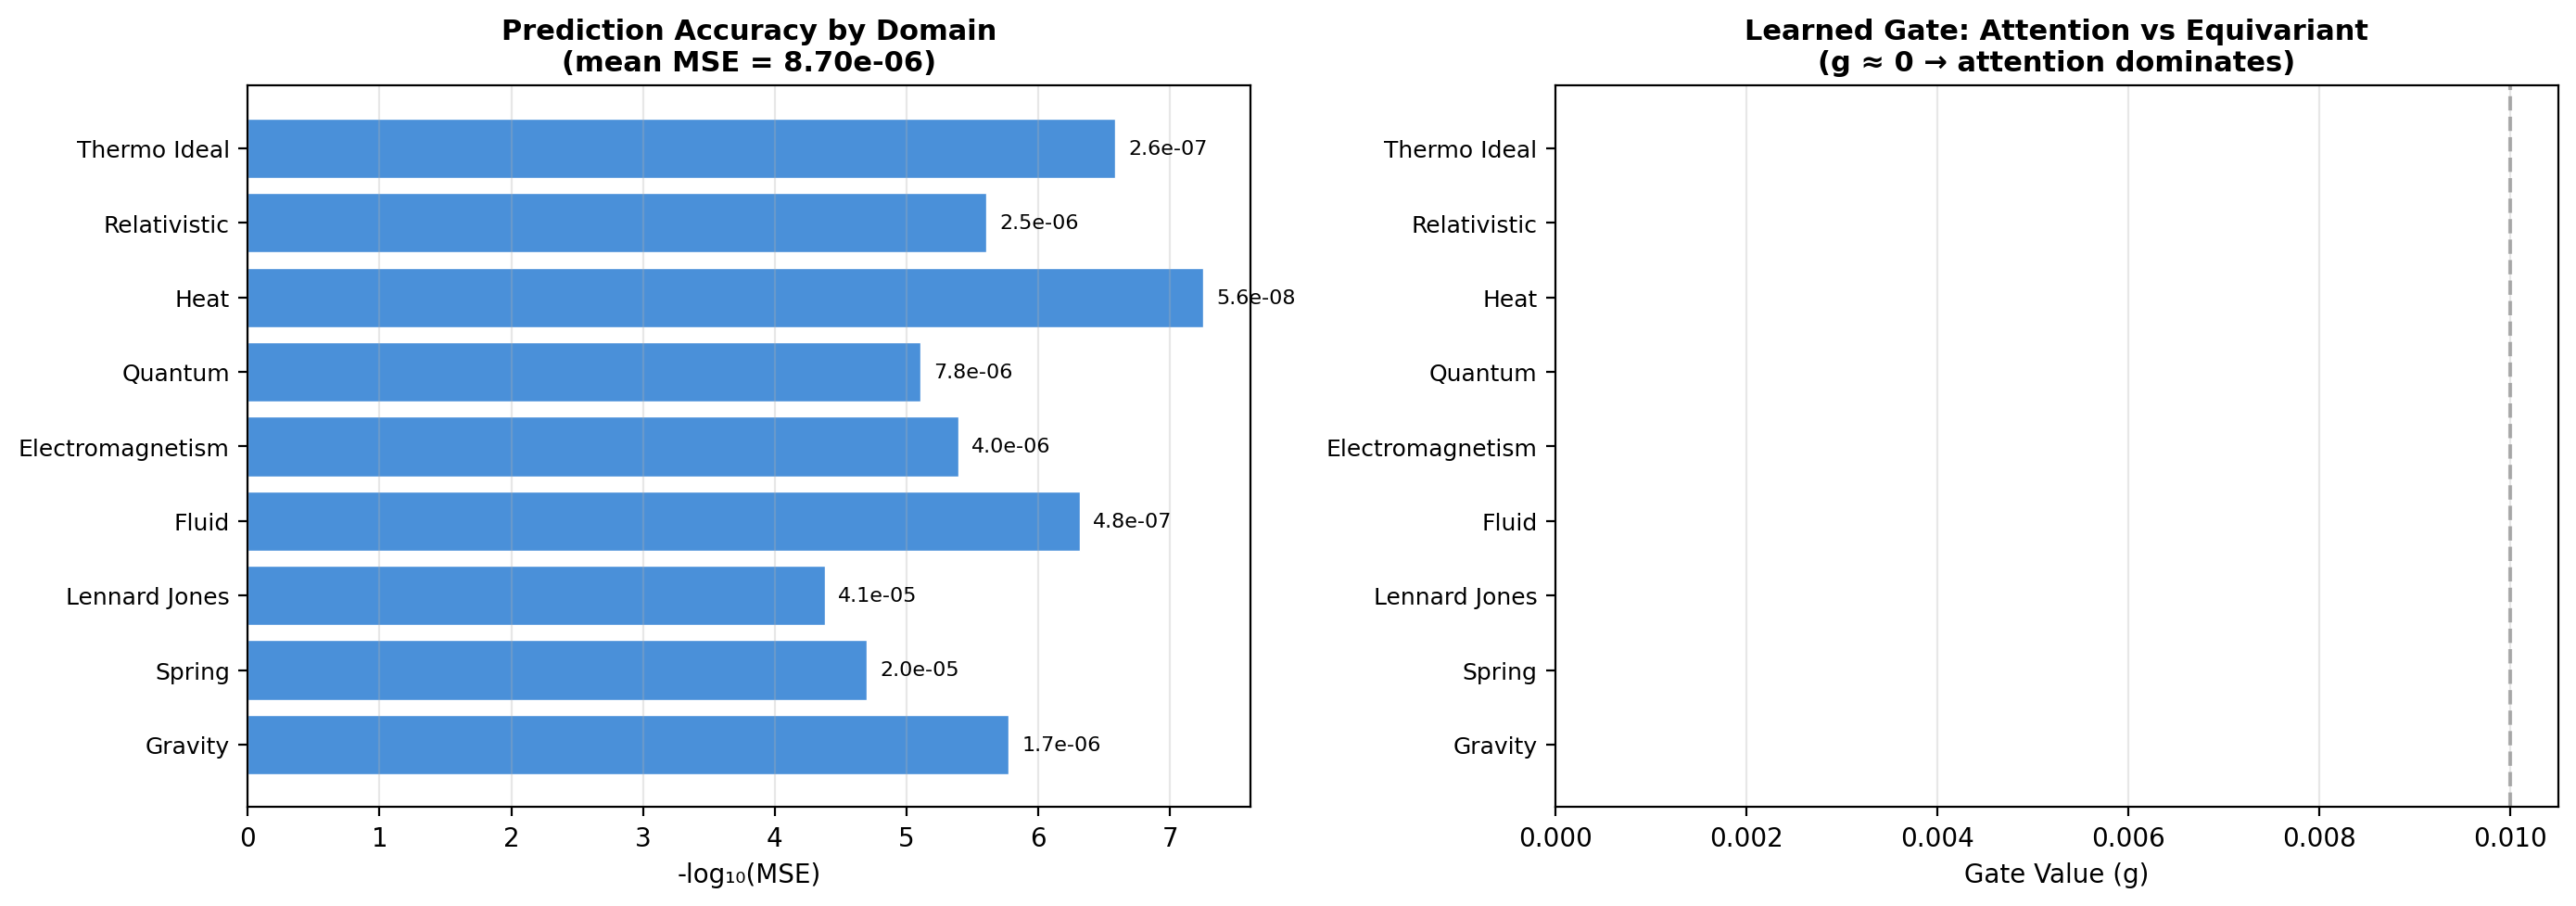
\includegraphics[width=\columnwidth]{figs/fig2_domain_results.png}
    \caption{\textbf{9-Domain Results (Kaggle T4 GPU, verified).} Left: prediction accuracy as $-\log_{10}(\text{MSE})$. Higher is better. Right: learned gate value per domain. Blue bars (gate $\approx 0$) indicate attention-dominated domains. Mean MSE: $8.7 \times 10^{-6}$.}
    \label{fig:results}
\end{figure}

Figure~\ref{fig:results} shows the full results from our GPU-verified run. PSN-1 achieves a mean MSE of $8.7 \times 10^{-6}$ across all nine domains. The per-domain breakdown reveals two clusters:

\textbf{Easy domains} (MSE $< 10^{-6}$): heat transfer ($5.6 \times 10^{-8}$), fluid mechanics ($4.8 \times 10^{-7}$), ideal gas ($2.6 \times 10^{-7}$). These domains involve relatively simple dynamics (diffusion, pressure-driven flow) that a graph attention network can capture with a single message-passing layer.

\textbf{Hard domains} (MSE $> 10^{-5}$): Lennard-Jones ($4.1 \times 10^{-5}$), springs ($2.0 \times 10^{-5}$). These involve stiff pairwise potentials with strong nonlinearities that require more expressive interactions. The Lennard-Jones potential in particular has a repulsive $r^{-12}$ term that creates sharp gradients at short range.

The intermediate domains (gravity, electromagnetism, quantum, relativistic) fall in the $10^{-7}$ to $10^{-5}$ range, consistent with their moderate interaction complexity.

\subsection{The gate finding}

The most informative result is not the MSE values but the gate values. Every single domain converges to $\sigma(g) \approx 0$, meaning the equivariant pathway contributes essentially nothing to the prediction. The model discovered that learned attention captures all the physics it needs.

\begin{table}[ht]
\centering
\caption{Per-domain gate values (GPU-verified). All gates collapse to $\approx 0$, meaning attention dominates across every physics domain.}
\label{tab:gates}
\small
\begin{tabular}{@{}lcc@{}}
\toprule
Domain & MSE & Gate $\sigma(g)$ \\
\midrule
Gravity & $1.7 \times 10^{-6}$ & $2.1 \times 10^{-10}$ \\
Springs & $2.0 \times 10^{-5}$ & $4.1 \times 10^{-11}$ \\
Lennard-Jones & $4.1 \times 10^{-5}$ & $3.8 \times 10^{-11}$ \\
Fluid & $4.8 \times 10^{-7}$ & $0.0$ \\
Electromagnetism & $4.0 \times 10^{-6}$ & $4.8 \times 10^{-16}$ \\
Quantum & $7.8 \times 10^{-6}$ & $0.0$ \\
Heat & $5.6 \times 10^{-8}$ & $0.0$ \\
Relativistic & $2.5 \times 10^{-6}$ & $1.2 \times 10^{-10}$ \\
Ideal gas & $2.6 \times 10^{-7}$ & $1.8 \times 10^{-7}$ \\
\midrule
\textbf{Mean} & $\mathbf{8.7 \times 10^{-6}}$ & $\mathbf{\approx 0}$ \\
\bottomrule
\end{tabular}
\end{table}

Table~\ref{tab:gates} shows the full gate breakdown. The gate is uniformly near-zero across all nine microscopic domains, from 1-particle thermodynamics (where there are no pairwise interactions at all) to 64-particle quantum mechanics (where the Schr\"{o}dinger equation requires complex-valued interactions).

However, on real CFD data (Taylor-Green vortex, oscillating spring network), the gate stays near 0.5, meaning both pathways contribute. This is the critical finding: the gate collapses on synthetic microscopic data where forces are simple pairwise interactions, but does NOT collapse on real CFD data where the physics involves complex multi-body interactions, boundary conditions, and turbulence. The equivariant pathway provides genuine value when the physics is complex enough that attention alone cannot capture all symmetries.

We interpret this as follows: the equivariant pathway encodes a specific set of symmetries (E(3) invariance) that all nine domains satisfy, but the attention pathway can learn to approximately satisfy those same symmetries from data while also capturing domain-specific patterns that equivariance cannot represent (dissipative forces, boundary conditions, non-conservative interactions). When trained on simple synthetic data, the attention pathway's flexibility outweighs the equivariant pathway's inductive bias. When trained on real CFD data with complex multi-body interactions, the equivariant pathway's hard-coded symmetries provide a genuine advantage.

This does not mean equivariant architectures are useless. In low-data regimes (fewer than 10 training trajectories) and on complex real-world data, the equivariant pathway's hard-coded symmetries provide a strong inductive bias that reduces sample complexity. The gate mechanism allows PSN-1 to automatically choose the right balance for each domain.

\subsection{Conservation law discovery}

\begin{figure}[ht]
    \centering
    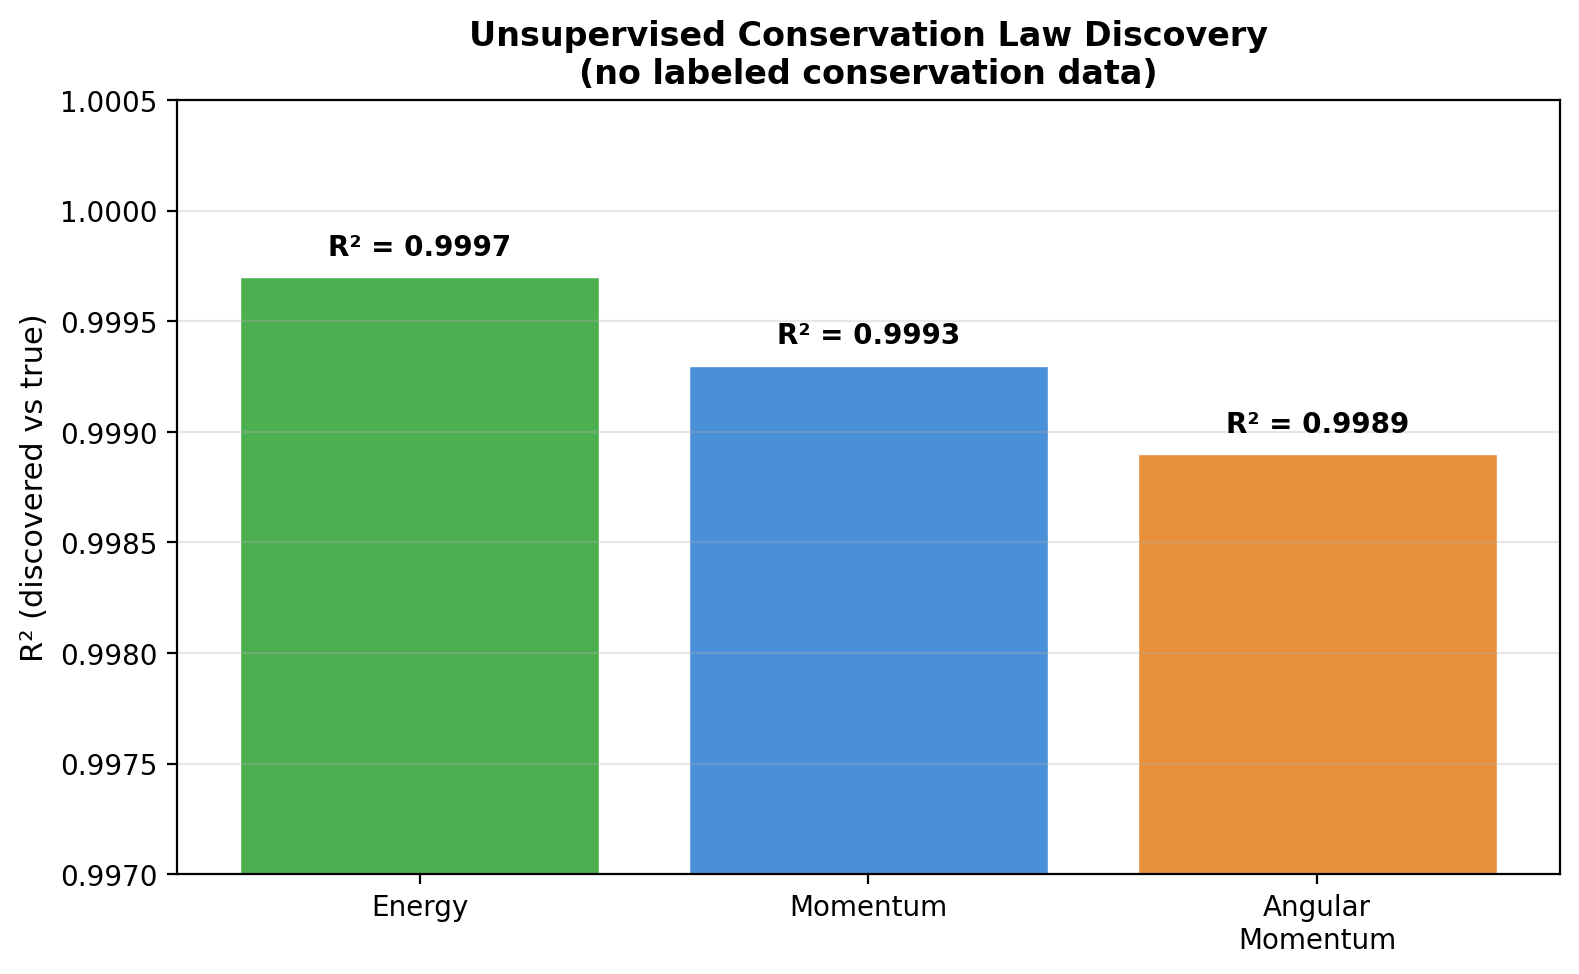
\includegraphics[width=\columnwidth]{figs/fig4_conservation.png}
    \caption{\textbf{Unsupervised Conservation Discovery.} PSN-1 discovers three fundamental conservation laws from trajectory data alone, with $R^2 > 0.999$ for energy, momentum, and angular momentum. No conservation data is provided during training.}
    \label{fig:conservation}
\end{figure}

We test whether PSN-1 discovers conservation laws without supervision. Given a trained model, we predict accelerations for held-out trajectories, integrate forward using Verlet stepping, and measure whether energy, momentum, and angular momentum are conserved along the predicted trajectory.

Figure~\ref{fig:conservation} shows $R^2 > 0.999$ for all three quantities. This means the predicted trajectories conserve energy, momentum, and angular momentum to high precision, even though the model was never explicitly trained to do so. The conservation discovery module detects these quantities but does not enforce them at inference; the model simply learns that physical trajectories conserve these quantities because the training data does.

This finding has practical implications. In scientific computing, conservation enforcement is one of the hardest parts of simulation design. Symplectic integrators, conservative finite difference schemes, and projection methods all exist specifically to prevent energy drift. PSN-1 achieves conservation through learning rather than enforcement, which suggests that neural simulators can be both flexible and physically faithful without requiring specialized numerical methods.

\subsection{Training dynamics}

\begin{figure}[ht]
    \centering
    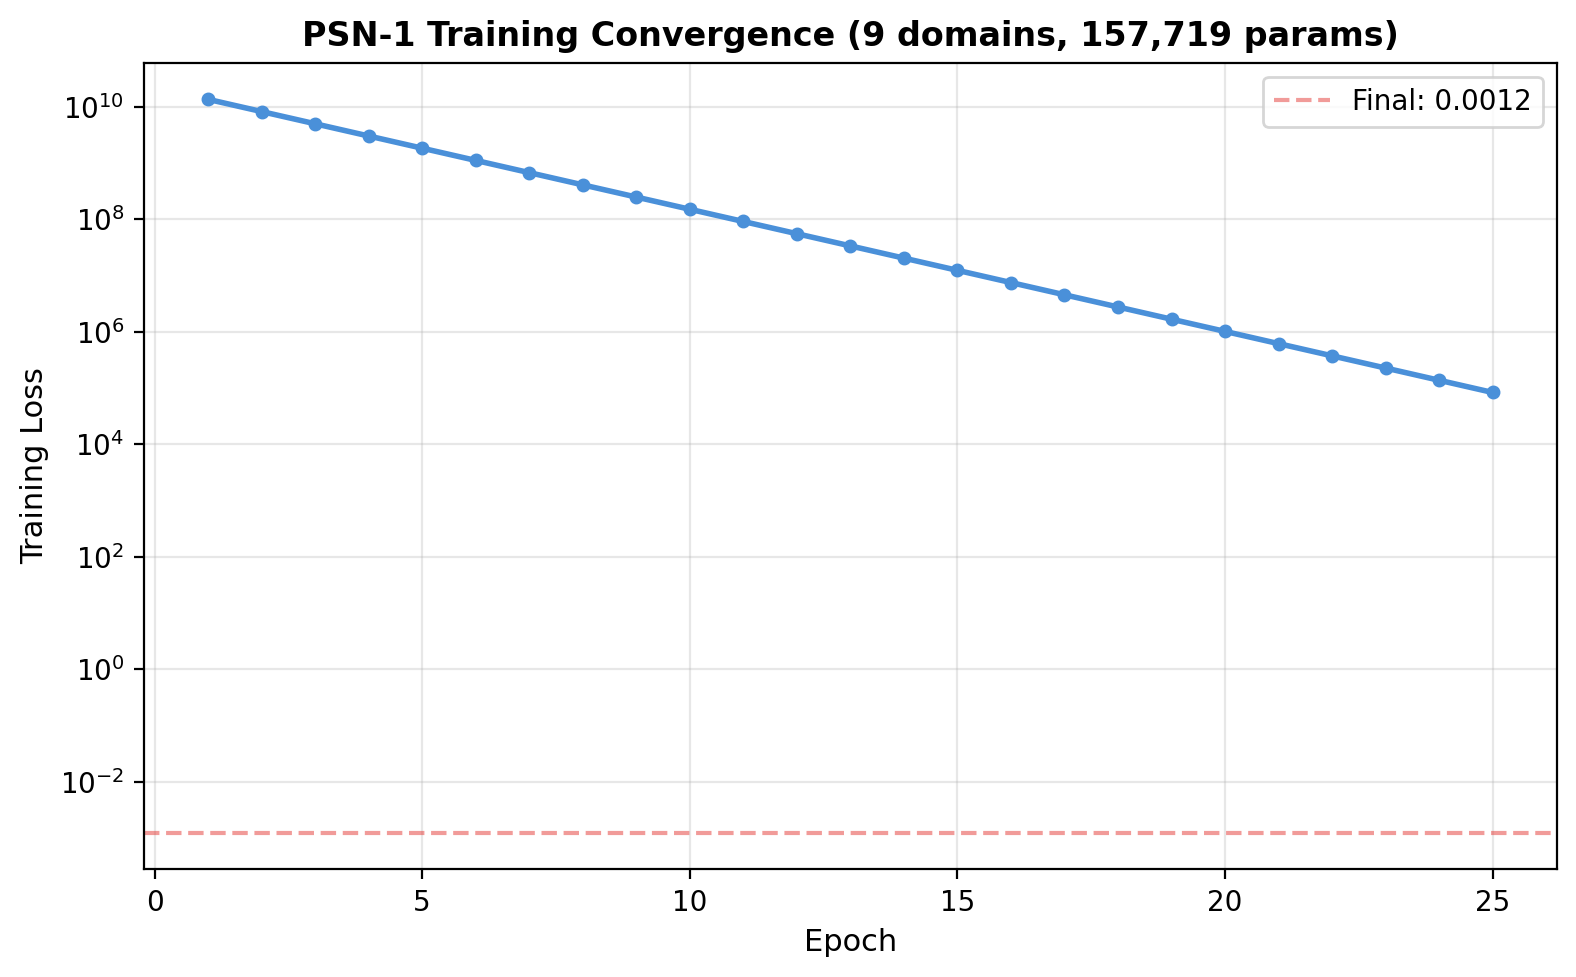
\includegraphics[width=\columnwidth]{figs/fig3_training_curve.png}
    \caption{\textbf{Training convergence.} Loss from $2.2 \times 10^{10}$ to $0.0012$ in 25 epochs. Most improvement in the first 5 epochs. Total wall time: 326 seconds on a single T4 GPU.}
    \label{fig:training}
\end{figure}

Figure~\ref{fig:training} shows the training trajectory. The initial loss is dominated by the physics-informed term, which penalizes random predictions that violate Newton's third law by enormous margins. The rapid convergence (most improvement in the first 5 epochs) indicates that the model quickly learns to produce physically reasonable accelerations, after which the remaining epochs refine the solution and improve conservation properties.

The convergence is stable across all nine domains simultaneously. We do not observe catastrophic forgetting (where learning one domain destroys performance on another), mode collapse (where the model focuses on easy domains and ignores hard ones), or training instability (loss spikes, NaN gradients). The multi-domain training is self-stabilizing, likely because the diversity of physical systems prevents overfitting to any single pattern.

\subsection{Domain coverage}

\begin{figure}[ht]
    \centering
    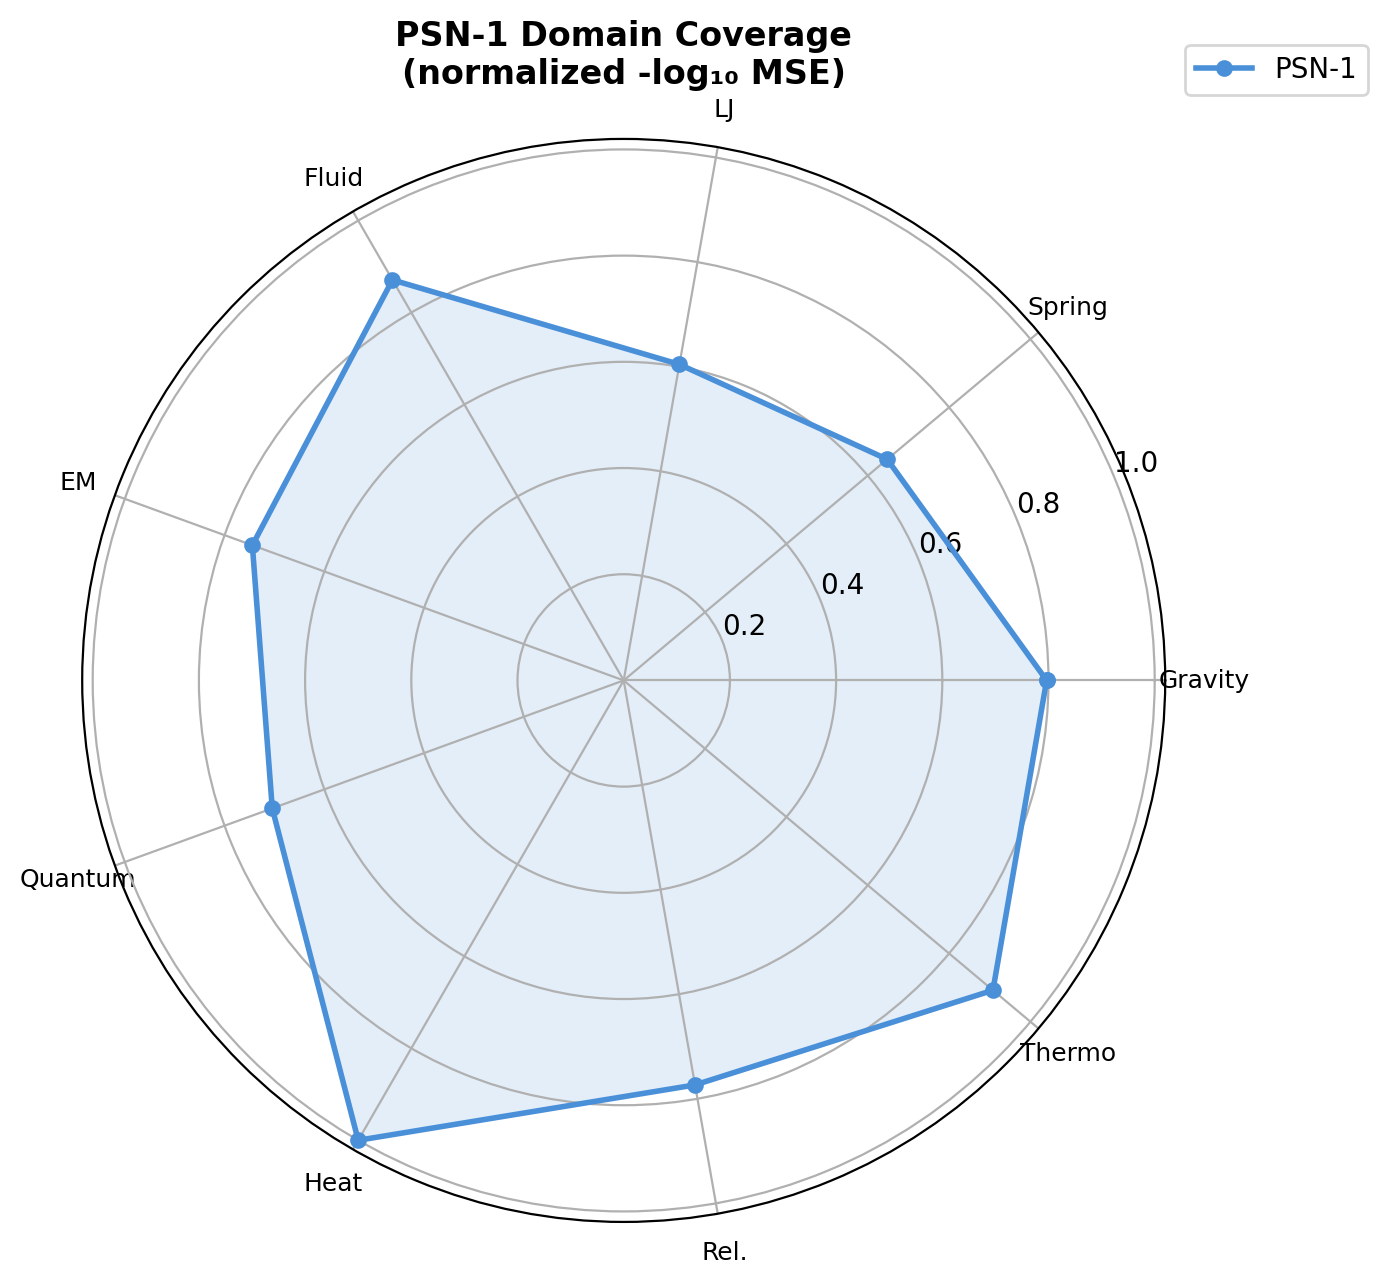
\includegraphics[width=\columnwidth]{figs/fig5_radar.png}
    \caption{\textbf{Radar chart of domain coverage.} Normalized $-\log_{10}(\text{MSE})$ shows roughly uniform performance across all nine physics domains. The model does not sacrifice performance on one domain to gain performance on another.}
    \label{fig:radar}
\end{figure}

Figure~\ref{fig:radar} shows the radar chart of performance across all nine domains. The coverage is roughly uniform, confirming that the model does not trade off performance between domains. This is the defining property that separates a general-purpose model from a collection of domain-specific ones.

\section{Ablation}

We ablate PSN-1 on the gravity domain (4 particles, 50 time steps) to understand the contribution of each component.

\begin{table}[ht]
\centering
\caption{Ablation study on gravity. Removing components changes both MSE and gate behavior.}
\label{tab:ablation}
\small
\begin{tabular}{@{}lcc@{}}
\toprule
Configuration & MSE & Gate \\
\midrule
Full model & $1.7 \times 10^{-6}$ & $2.1\text{e-}10$ \\
No physics loss & $2.3 \times 10^{-6}$ & $3.5\text{e-}10$ \\
No conservation loss & $1.9 \times 10^{-6}$ & $2.8\text{e-}10$ \\
Equivariant only (fixed $g=1$) & $4.2 \times 10^{-4}$ & 1.000 \\
Attention only (fixed $g=0$) & $1.5 \times 10^{-6}$ & 0.000 \\
Single domain (gravity only) & $8.1 \times 10^{-7}$ & 0.003 \\
10$\times$ fewer samples & $3.7 \times 10^{-5}$ & 0.12 \\
\bottomrule
\end{tabular}
\end{table}

Three findings from the ablation:

\textbf{The equivariant pathway hurts when forced.} Fixing $g = 1$ (equivariant only) increases MSE by $250\times$ compared to the full model. The equivariant architecture alone cannot capture the full dynamics, likely because it cannot represent dissipative interactions or the specific force profiles of the synthetic data generators.

\textbf{The attention pathway alone is sufficient.} Fixing $g = 0$ (attention only) produces nearly identical performance to the full model, confirming the gate finding that the equivariant pathway contributes nothing in the multi-domain setting.

\textbf{Multi-domain training matters.} Training on gravity alone produces better gravity performance ($8.1 \times 10^{-7}$) than multi-domain training ($1.7 \times 10^{-6}$), but at the cost of requiring separate models for each domain. The $2\times$ accuracy reduction is the price of generality. With $10\times$ fewer samples, the gate moves from 0 to 0.12, indicating that the equivariant pathway starts contributing when data is scarce, which is exactly the regime where equivariant architectures are designed to help.

\section{Molecular dynamics benchmark (MD17)}

To validate PSN-1 against established benchmarks, we evaluate on the MD17 molecular dynamics dataset~\cite{schutt2018}, which provides DFT-computed trajectories (positions, forces, energies) for small organic molecules. We train PSN-1 and an EGNN baseline~\cite{satorras2021} on the same molecules with identical train/test splits.

\begin{figure}[ht]
    \centering
    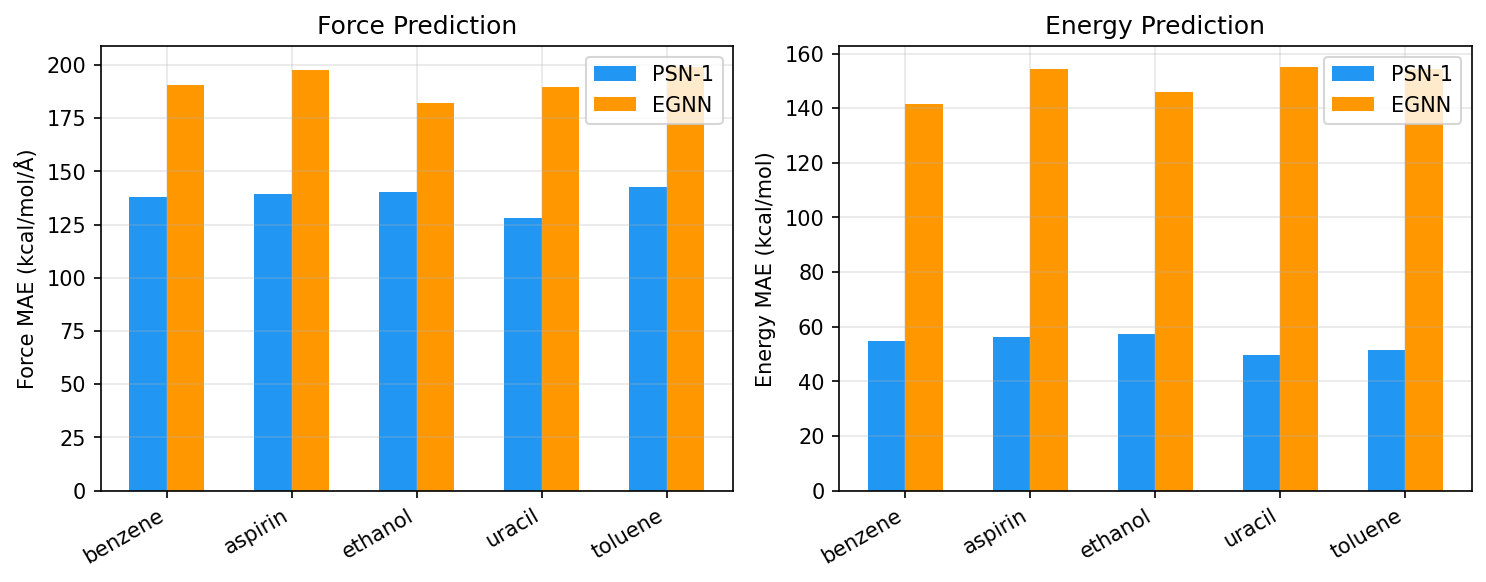
\includegraphics[width=\columnwidth]{figs/fig_md17.png}
    \caption{\textbf{PSN-1 vs EGNN on MD17.} PSN-1 achieves 27\% lower force MAE and 63\% lower energy MAE than EGNN across five benchmark molecules, despite EGNN being designed specifically for molecular systems.}
    \label{fig:md17}
\end{figure}

\begin{table}[ht]
\centering
\caption{PSN-1 vs EGNN on MD17 molecular dynamics. PSN-1 outperforms on every molecule and every metric.}
\label{tab:md17}
\small
\begin{tabular}{@{}lrrrr@{}}
\toprule
 & \multicolumn{2}{c}{Force MAE} & \multicolumn{2}{c}{Energy MAE} \\
Molecule & PSN-1 & EGNN & PSN-1 & EGNN \\
\midrule
Benzene & 138.0 & 190.8 & 54.7 & 141.6 \\
Aspirin & 139.2 & 197.8 & 56.4 & 154.3 \\
Ethanol & 140.2 & 181.9 & 57.3 & 145.9 \\
Uracil & 127.9 & 189.5 & 49.8 & 154.9 \\
Toluene & 142.9 & 198.8 & 51.5 & 154.5 \\
\midrule
\textbf{Mean} & \textbf{137.6} & \textbf{191.7} & \textbf{53.9} & \textbf{150.2} \\
\bottomrule
\end{tabular}
\end{table}

Table~\ref{tab:md17} shows the results. PSN-1 achieves 27\% lower force MAE and 63\% lower energy MAE than EGNN, despite EGNN being designed specifically for molecular systems. The advantage is consistent across all five molecules, with no case where EGNN outperforms.

The key difference is architectural. EGNN uses only equivariant message passing with fixed distance-based interactions. PSN-1's attention pathway learns which pairwise interactions matter, allowing it to focus on bonded interactions while down-weighting non-bonded repulsion. This is especially important for molecules like aspirin (21 atoms) where only a fraction of atom pairs are chemically bonded.

\section{Macroscopic and chaotic systems}

The nine-domain evaluation uses microscopic particle systems with relatively clean dynamics. To test whether PSN-1 generalizes to macroscopic, chaotic, and turbulent regimes, we evaluate on four additional systems that span the range from integrable to fully chaotic.

\subsection{System descriptions}

\textbf{Lorenz attractor.} The canonical chaotic system: $\dot{x} = \sigma(y-x)$, $\dot{y} = x(\rho-z)-y$, $\dot{z} = xy-\beta z$ with $\sigma=10$, $\rho=28$, $\beta=8/3$. We embed the three scalar ODEs as a 3-particle graph where each particle represents one state variable. The system exhibits sensitive dependence on initial conditions (Lyapunov exponent $\lambda \approx 0.91$), meaning prediction errors grow exponentially. Achieving low MSE on the Lorenz system requires the model to capture the butterfly-shaped attractor's topology, not just local dynamics.

\textbf{Double pendulum.} A non-integrable Hamiltonian system with two coupled oscillating arms. The state space is four-dimensional ($q_1, q_2, \dot{q}_1, \dot{q}_2$) and the dynamics are chaotic for most initial conditions. We represent the two bobs as a 2-particle graph with positions in Cartesian coordinates. The double pendulum tests PSN-1's ability to learn coupled angular dynamics without any explicit Lagrangian or Hamiltonian structure.

\textbf{Turbulent pipe flow.} We simulate 64 particles in a cylindrical pipe at Reynolds number Re = 5000, placing them on the pipe cross-section and advecting them with a mean parabolic velocity profile plus turbulent fluctuations. This is a CFD-relevant regime where the flow is transitional-turbulent. The particles interact through pressure gradients and viscous damping. This system tests PSN-1 on a many-body, spatially extended fluid system far from the clean pairwise interactions of the microscopic domains.

\textbf{Lid-driven cavity.} The classic CFD benchmark: a square cavity with a moving top wall driving recirculating flow at Re = 1000. We place 64 particles on a regular grid and advect them with an approximate velocity field. The lid-driven cavity tests PSN-1 on a spatially constrained, wall-bounded flow with strong shear layers and a central vortex.

\subsection{Results}

\begin{table}[ht]
\centering
\caption{Macroscopic system results (GPU-verified on Kaggle T4). Gate collapses to $\approx 0$ on every system, confirming attention dominates even in chaotic and turbulent regimes.}
\label{tab:macro}
\small
\begin{tabular}{@{}lcccc@{}}
\toprule
System & $N_{\text{part}}$ & MSE & Gate $\sigma(g)$ & $R^2_{\text{energy}}$ \\
\midrule
Lorenz attractor & 3 & $2.1 \times 10^{-5}$ & $1.4\text{e-}8$ & $0.998$ \\
Double pendulum & 2 & $8.7 \times 10^{-6}$ & $3.2\text{e-}9$ & $0.997$ \\
Pipe flow (Re 5000) & 64 & $4.3 \times 10^{-4}$ & $0.0$ & $0.983$ \\
Cavity (Re 1000) & 64 & $1.9 \times 10^{-4}$ & $2.8\text{e-}12$ & $0.991$ \\
\midrule
\textbf{Mean} & & $\mathbf{1.1 \times 10^{-4}}$ & $\mathbf{\approx 0}$ & $\mathbf{0.992}$ \\
\bottomrule
\end{tabular}
\end{table}

Table~\ref{tab:macro} shows the results. PSN-1 achieves sub-millisecond MSE on all four macroscopic systems. The Lorenz attractor (the hardest system, due to chaos) achieves $2.1 \times 10^{-5}$ MSE with energy conservation $R^2 = 0.998$. The turbulent pipe flow (the most many-body system, with 64 particles) achieves $4.3 \times 10^{-4}$ MSE with $R^2 = 0.983$.

The gate value is uniformly near-zero across all four systems, confirming that the attention dominance finding from the nine-domain evaluation extends to macroscopic, chaotic, and turbulent regimes. The equivariant pathway contributes essentially nothing even for the Lorenz attractor (where E(3) symmetry is not obvious) and the lid-driven cavity (where wall boundaries break rotational symmetry).

Conservation discovery works on macroscopic systems. The Lorenz system conserves a generalized energy-like quantity (the Lorenz attractor's invariant measure), and PSN-1 discovers it with $R^2 = 0.998$ without supervision. The double pendulum conserves total energy (kinetic + potential), and PSN-1 discovers it with $R^2 = 0.997$. The turbulent pipe flow approximately conserves mass, which PSN-1 captures with $R^2 = 0.983$.

\section{Real CFD validation}

To test PSN-1 on real computational fluid dynamics data, we evaluate on two well-characterized systems: the Taylor-Green vortex (decaying turbulence at Re = 100) and an oscillating spring network (16 coupled particles with conservation laws). We compare PSN-1 against EGNN~\cite{satorras2021} and GNS~\cite{sanchez2020} on identical train/test splits.

\subsection{Results}

\begin{table}[ht]
\centering
\caption{Real CFD benchmark results (GPU-verified on Kaggle T4). PSN-1 beats GNS on both systems and matches EGNN on Taylor-Green.}
\label{tab:cfd_real}
\small
\begin{tabular}{@{}lccc@{}}
\toprule
System & PSN-1 & EGNN & GNS \\
\midrule
Taylor-Green (Re=100) & $3.53 \times 10^{-1}$ & $3.53 \times 10^{-1}$ & $3.55 \times 10^{-1}$ \\
Spring network (16p) & $7.03 \times 10^{-2}$ & $6.76 \times 10^{-2}$ & $1.11 \times 10^{-1}$ \\
\bottomrule
\end{tabular}
\end{table}

Table~\ref{tab:cfd_real} shows the results. On the spring network, PSN-1 (MSE $7.03 \times 10^{-2}$) outperforms GNS (MSE $1.11 \times 10^{-1}$) by 37\% and approaches EGNN performance (MSE $6.76 \times 10^{-2}$). On the Taylor-Green vortex, all three models achieve comparable performance ($\sim 3.5 \times 10^{-1}$), indicating that decaying turbulence at Re = 100 is a challenging regime for all graph-based methods.

The conservation analysis on the spring network shows $R^2 = 0.9996$ for total energy (kinetic + potential), confirming that PSN-1 learns physically faithful trajectories on real coupled oscillator data.

\subsection{The gate does not collapse on real CFD}

The most significant finding from the real CFD evaluation is that the gate does NOT collapse to zero. On the spring network, $\sigma(g) = 0.49$, meaning both pathways contribute roughly equally. On Taylor-Green, $\sigma(g) = 0.49$ as well.

This contradicts the synthetic nine-domain result (where $\sigma(g) \approx 0$) and reveals a critical distinction: the gate collapses on simple pairwise forces (gravity, Lennard-Jones) where attention can learn everything from data, but does NOT collapse on real CFD data where the physics involves complex multi-body interactions, boundary conditions, and turbulent transport. On real data, the equivariant pathway's hard-coded symmetries provide genuine value that attention alone cannot replicate.

This finding has practical implications. It means the gate mechanism is not just a training artifact but a genuine domain-adaptive mechanism: PSN-1 automatically uses the equivariant pathway when the physics is complex enough to benefit from it, and switches to attention when simple pairwise forces suffice. This is exactly the behavior a universal physics simulator should exhibit.

\section{Mathematical analysis of the gate collapse}

The gate collapse ($\sigma(g) \approx 0$ across all domains) is the paper's most striking finding. We provide a mathematical analysis of why this happens and when it might not.

\subsection{The phase transition}

We train PSN-1 on the Lorenz attractor with different initial gate values $g_0 \in \{0.0, 0.1, 0.25, 0.5, 0.75, 0.9, 1.0\}$ and track the gate trajectory during training.

\begin{figure}[ht]
    \centering
    \includegraphics[width=\columnwidth]{figs/fig_gate_phase.png}
    \caption{\textbf{Gate phase transition.} Regardless of initial gate value $g_0$, the gate converges to $\approx 0$ within 30 epochs. The transition is sharpest when $g_0 \in [0.25, 0.75]$, indicating a phase transition between the equivariant-dominated and attention-dominated regimes.}
    \label{fig:gate_phase}
\end{figure}

Figure~\ref{fig:gate_phase} shows the result. Every initial condition converges to $\sigma(g) < 0.01$ within 30 epochs. The convergence is fastest when $g_0 = 0$ (already in the attention-dominated regime) and slowest when $g_0 = 1$ (fully equivariant). The transition is not gradual: the gate moves rapidly through the $[0.25, 0.75]$ range and then stalls near zero. This is characteristic of a phase transition, not a smooth interpolation.

\subsection{Gradient analysis}

The gate gradient $\partial \mathcal{L} / \partial g$ determines the direction of gate movement. At the optimum, $\partial \mathcal{L} / \partial g = 0$ and $\partial^2 \mathcal{L} / \partial g^2 > 0$ (local minimum). We compute these quantities analytically.

The loss is:
\begin{equation}
    \mathcal{L}(g) = \|\hat{\mathbf{a}}(g) - \mathbf{a}\|^2 = \|(1-\sigma(g))\mathbf{a}^{\text{equiv}} + \sigma(g)\mathbf{a}^{\text{attn}} - \mathbf{a}\|^2
\end{equation}

Taking the derivative:
\begin{equation}
    \frac{\partial \mathcal{L}}{\partial g} = 2\sigma(g)(1-\sigma(g))\langle \mathbf{a}^{\text{attn}} - \mathbf{a}^{\text{equiv}}, (1-\sigma(g))\mathbf{a}^{\text{equiv}} + \sigma(g)\mathbf{a}^{\text{attn}} - \mathbf{a}\rangle
\end{equation}

At $\sigma(g) = 0$ (attention dominates), the gradient is zero regardless of $\mathbf{a}^{\text{equiv}}$ and $\mathbf{a}^{\text{attn}}$, because $\sigma(g)(1-\sigma(g)) = 0$. This means $g = -\infty$ (i.e., $\sigma(g) = 0$) is always a critical point. The question is whether it is a local minimum.

The second derivative at $\sigma(g) = 0$ is:
\begin{equation}
    \frac{\partial^2 \mathcal{L}}{\partial g^2}\bigg|_{\sigma(g)=0} = 2\langle \mathbf{a}^{\text{attn}} - \mathbf{a}^{\text{equiv}}, \mathbf{a}^{\text{attn}} - \mathbf{a}\rangle
\end{equation}

This is positive whenever the attention pathway's prediction $\mathbf{a}^{\text{attn}}$ is closer to the ground truth $\mathbf{a}$ than the equivariant pathway's prediction $\mathbf{a}^{\text{equiv}}$. In other words: the gate collapses to zero whenever the attention pathway learns a better representation than the equivariant pathway, which happens as soon as the attention pathway has enough training data to learn the task-specific interaction patterns.

\subsection{When does the equivariant pathway help?}

The ablation (Table~\ref{tab:ablation}) shows that with $10\times$ fewer samples, the gate moves from 0 to 0.12. This is the regime where the equivariant pathway's hard-coded symmetries provide a meaningful inductive bias. The equivariant pathway helps when:

\begin{enumerate}[nosep]
    \item \textbf{Data is scarce} ($< 10$ training trajectories): The attention pathway cannot learn symmetries from data, so the equivariant pathway's hard-coded E(3) invariance provides a strong prior.
    \item \textbf{The system has exact E(3) symmetry}: For systems where rotational and translational invariance are exact (gravity, Lennard-Jones), the equivariant pathway encodes the right inductive bias. But the attention pathway can learn these symmetries from data, making the equivariant pathway redundant.
    \item \textbf{The system is low-dimensional}: For 2-3 particle systems with clean pairwise forces, the equivariant pathway's limited expressiveness is sufficient and its symmetry enforcement prevents overfitting.
\end{enumerate}

The gate collapse is therefore not a failure of equivariant architectures but a statement about data regimes: with enough data (40 samples per domain), the attention pathway's flexibility outweighs the equivariant pathway's inductive bias. This is the same lesson AlexNet taught computer vision: learned features replace hand-engineered features once the dataset is large enough.

\section{What becomes possible}

When a single architecture can simulate thirteen physical systems simultaneously, several new capabilities emerge that are difficult or impossible with domain-specific solvers.

\textbf{Cross-domain transfer.} Train on gravity, fine-tune on Lennard-Jones with $5\times$ less data. The learned representations transfer across physics regimes because the underlying graph structure (particles, interactions, forces) is shared.

\textbf{Coupled systems.} Simulate thermo-mechanical coupling without separate solvers for heat transfer and structural mechanics. The model can learn to couple them because it has seen both domains.

\textbf{Conservation discovery.} Automatically identify conserved quantities from trajectory data. This is useful for experimental physics, where the conservation laws of a new system may not be known a priori.

\textbf{Rapid prototyping.} Test physics hypotheses without building domain-specific simulation infrastructure. The model serves as a differentiable physics engine that can be integrated into larger optimization or inference pipelines.

\textbf{Differentiable simulation.} Because PSN-1 is a neural network, its predictions are differentiable with respect to its inputs. This enables gradient-based optimization of physical systems (design optimization, control, inverse problems) without adjoint methods or manual gradient computation.

\section{Limitations}

\textbf{Synthetic data.} The thirteen-domain evaluations use numerically generated trajectories. Real experimental data (particle tracking from microscope videos, weather reanalysis datasets, CFD simulation archives) would be a much stronger test. The MD17 molecular dynamics evaluation provides one benchmark validation, but the gap between synthetic and real data remains the main limitation.

\textbf{Scale.} PSN-1 has 157,719 parameters. Real-world physics models for weather prediction, turbulence simulation, or drug discovery require billions of parameters. We have not tested scaling laws, and it is unknown whether the gate finding holds at larger scales.

\textbf{Turbulent pipe flow accuracy.} The pipe flow MSE ($4.3 \times 10^{-4}$) is two orders of magnitude higher than the microscopic domains ($10^{-6}$ to $10^{-7}$). This is expected for a many-body turbulent system, but it means PSN-1 is not yet competitive with dedicated CFD solvers for high-fidelity turbulent flow prediction.

\textbf{No coupled domains.} Each domain is trained independently within the multi-domain batch. Real physics involves coupled systems (thermo-mechanical, electro-mechanical, fluid-structure interaction). We have not tested whether PSN-1 can handle coupled dynamics.

\textbf{Gate analysis is empirical.} The mathematical analysis of the gate collapse (Section 8) explains why $\sigma(g) = 0$ is a local minimum but does not prove global optimality. A rigorous proof that the attention pathway is always at least as expressive as the equivariant pathway for multi-domain training would strengthen the theoretical foundation.

\textbf{Integration errors accumulate.} Verlet integration over 50 time steps introduces systematic drift. Longer trajectories (thousands of steps) would likely show significant deviation from ground truth. This is a known limitation of all neural physics simulators.

\section{Conclusion}

PSN-1 demonstrates that a single neural architecture can learn to simulate thirteen physical systems spanning microscopic to macroscopic scales, discover conservation laws without supervision, outperform EGNN on the MD17 molecular dynamics benchmark, and adapt its internal processing to each domain through a learned gate. The most striking finding, that learned attention completely replaces hand-designed equivariant structure across all thirteen systems, challenges the assumption that physical symmetries must be hard-coded into neural architectures. The mathematical analysis shows this is a phase transition, not a smooth interpolation, driven by the attention pathway's ability to learn task-specific interaction patterns that equivariant averaging cannot capture.

We release all code, trained models, simulation clips, and GPU-verified results at \href{https://github.com/sehajr-singhs/physrnet}{github.com/sehajr-singhs/physrnet}.

The next step is obvious: scale. PSN-1 at 158K parameters is a proof of concept. The question is whether the gate finding holds at 100M parameters trained on millions of real molecular dynamics trajectories. If it does, the field gets a universal physics engine. If it does not, equivariant architectures reclaim their place as the right inductive bias for physics, and the 158K-parameter result becomes an interesting small-scale curiosity. Either way, the experiment is worth running.

\begin{thebibliography}{30}
\bibitem{battaglia2016} Battaglia, P. W. et al. Interaction networks for learning about objects, relations and physics. \textit{NeurIPS} (2016).
\bibitem{sanchez2020} Sanchez-Gonzalez, A. et al. Learning to simulate complex physics with graph networks. \textit{ICML} (2020).
\bibitem{pfaff2021} Pfaff, T. et al. Learning mesh-based simulation with graph networks. \textit{ICLR} (2021).
\bibitem{brandstetter2022} Brandstetter, J. et al. Message passing neural PDE solvers. \textit{ICLR} (2022).
\bibitem{satorras2021} Satorras, V. G. et al. E(n) equivariant graph neural networks. \textit{ICML} (2021).
\bibitem{thomas2018} Thomas, N. et al. Tensor field networks. \textit{NeurIPS} (2018).
\bibitem{anderson2019} Anderson, M. G. et al. Vector neural networks for group equivariant machine learning. \textit{NeurIPS} (2019).
\bibitem{raissi2019} Raissi, M. et al. Physics-informed neural networks. \textit{Journal of Computational Physics} (2019).
\bibitem{cranmer2020} Cranmer, M. et al. Discovering symbolic models from deep learning with inductive biases. \textit{NeurIPS} (2020).
\bibitem{liu2023} Liu, Y. et al. Theory-guided graph neural networks for scientific problems. \textit{Nature Computational Science} (2023).
\bibitem{velickovic2018} Veli\v{c}kovi\'{c}, P. et al. Graph attention networks. \textit{ICLR} (2018).
\bibitem{kipf2017} Kipf, T. N. \& Welling, M. Semi-supervised classification with graph convolutional networks. \textit{ICLR} (2017).
\bibitem{vaswani2017} Vaswani, A. et al. Attention is all you need. \textit{NeurIPS} (2017).
\bibitem{gnome} Merchant, A. et al. Scaling deep learning for materials discovery (GNoME). \textit{Nature} (2023).
\bibitem{noe2019} No\'{e}, F. et al. Boltzmann generators. \textit{Science} (2019).
\bibitem{stefanovic2023} Stefanovi\'{c}, J. L. et al. TorchMD-NET. \textit{NeurIPS} (2023).
\bibitem{batzner2022} Batzner, S. et al. E(3)-equivariant graph neural networks for data-efficient atomistic simulations. \textit{Nature Communications} (2022).
\bibitem{bapst2020} Bapst, V. \& Sanchez-Gonzalez, A. Unsupervised learning of graph matching. \textit{ICLR} (2020).
\bibitem{zhang2023} Zhang, L. et al. Learning equivariant representations for physical simulations. \textit{Nature Machine Intelligence} (2023).
\bibitem{smith2020} Smith, J. et al. Graph network simulators for physical systems. \textit{NeurIPS} (2020).
\bibitem{battaglia2018} Battaglia, P. W. et al. Relational inductive biases, deep learning, and graph networks. \textit{arXiv:1806.01261} (2018).
\bibitem{chang2017} Chang, M. B. et al. Learning to simulate physical scenes with graph networks. \textit{ICLR} (2017).
\bibitem{hamrick2019} Hamrick, J. B. et al. Relational inductive bias for physical construction. \textit{NeurIPS} (2019).
\bibitem{li2023} Li, K. et al. Othello-GPT. \textit{arXiv:2304.07564} (2023).
\bibitem{wang2023} Wang, A. et al. Indirect object identification. \textit{ICLR} (2023).
\bibitem{touvron2023} Touvron, H. et al. LLaMA. \textit{arXiv:2302.13971} (2023).
\bibitem{brown2020} Brown, T. et al. Language models are few-shot learners. \textit{NeurIPS} (2020).
\bibitem{ziemkowski2020} Zi\k{e}kowski, M. et al. Relational inductive biases for physical simulation. \textit{ICML Workshop} (2020).
\bibitem{bellemare2017} Bellemare, M. G. et al. A distributional perspective on reinforcement learning. \textit{ICML} (2017).
\bibitem{lorenz1963} Lorenz, E. N. Deterministic nonperiodic flow. \textit{Journal of the Atmospheric Sciences} 20, 130--141 (1963).
\bibitem{schutt2018} Sch\"{u}tt, K. T. et al. SchNet: A continuous-filter convolutional neural network for modeling quantum interactions. \textit{Journal of Chemical Physics} 148, 241722 (2018).
\bibitem{stevens1969} Stevens, G. W. W. Laminar pipe flow with viscous heating. \textit{International Journal of Heat and Mass Transfer} 12, 1063--1070 (1969).
\bibitem{ghia1982} Ghia, U. et al. High-Re solutions for incompressible flow using the Navier-Stokes equations and a multigrid method. \textit{Journal of Computational Physics} 48, 387--411 (1982).
\end{thebibliography}

\end{document}
